\documentclass{article}
\usepackage[margin=2cm]{geometry}
\usepackage{graphicx}
\usepackage[pages=some]{background}
\usepackage{titling}
\usepackage{tabularx}
\usepackage{tikz}
\usepackage{subfigure}
\usepackage{multicol}
\usepackage{caption}

\geometry{a4paper}

\backgroundsetup{
    scale=1,
    angle=0,
    opacity=1,
    contents={%
        
\includegraphics[width=\paperwidth,height=\paperheight]{institution_logo.jpg}
    }
}

\newcommand{\subtitle}[1]{
    \posttitle{
        \par\end{center}
        \begin{center}\large#1\end{center}
        \vskip0.5em}
}

\title{IPE-431}
\author{Md. Hasibul Islam}
\subtitle{MACHINE TOOLS}

\begin{document}
\begin{titlepage}
    \centering
    
    {\Huge\bfseries\maketitle}
    \textbf{Rashik Ahnaf Sir} \\
    \vspace{2cm}
    
\includegraphics[width=8cm]{institution_logo.jpg}
    \vfill
    \vspace*{2cm}
\end{titlepage}

\tableofcontents
\pagebreak
\section{Lecture 01: Engine Lathe} 
\hfill Date: 05/06/2023

\subsection*{Booklist}

\textbf{Machine Tools by N. Chernov}


\subsection*{Engine Lathe}
An engine lathe, also known as a center lathe or a turning lathe, is a type of machine tool used in metalworking processes to shape and cut metal workpieces. A machine tool used for machining of mainly cylindrical workpieces. It is one of the most commonly used lathes in manufacturing and repair shops. Engine lathes are versatile machines capable of performing a wide range of operations, including \textbf{facing, centering, turning, threading, parting, drilling, boring, chamfering, knurling.}  Both external and internal operations can be performed.


\subsubsection*{Components of Engine Lathe}
The basic components of an engine lathe include a bed, headstock, tailstock, carriage, tool post, and various controls. Let's explore each component in more detail:
\begin{itemize}
  \item \textbf{Bed}: The bed is the main base of the lathe and provides a rigid and stable platform for supporting other components. It is usually made of cast iron and has a flat, horizontal surface on which the workpiece rests. The bed contains guideways or V-ways that guide the movement of the carriage along the length of the lathe.
  \item \textbf{Headstock}: The headstock is located on one end of the bed and houses the main spindle. The spindle is driven by a motor and provides the rotational motion to the workpiece. It also contains a variety of speed and feed controls to adjust the cutting speed and direction.
  \item \textbf{Tailstock}: The tailstock is located on the other end of the bed and is movable along the bed's guideways. It consists of a spindle, which can be extended or retracted, and is used to support the other end of the workpiece. The tailstock often includes a center or a chuck for gripping the workpiece securely.
  \item \textbf{Carriage}: The carriage is mounted on the bed and can move along the length of the lathe using the guideways. It consists of several components, including the saddle, cross-slide, and apron. The carriage carries the cutting tool and controls its movement across the workpiece.
  \item \textbf{Tool Post}: The tool post is located on top of the carriage and holds the cutting tool securely. It allows for quick and easy tool changes, enabling the operator to use different tools for various operations.
  \item \textbf{Controls}: The engine lathe has a variety of controls to regulate the speed, feed, and direction of the cutting tool. These controls can be manual or automated, depending on the lathe's design and features. They enable the operator to adjust the cutting parameters according to the workpiece material and desired machining outcome.
\end{itemize}

\begin{figure}[htbp]
  \centering
  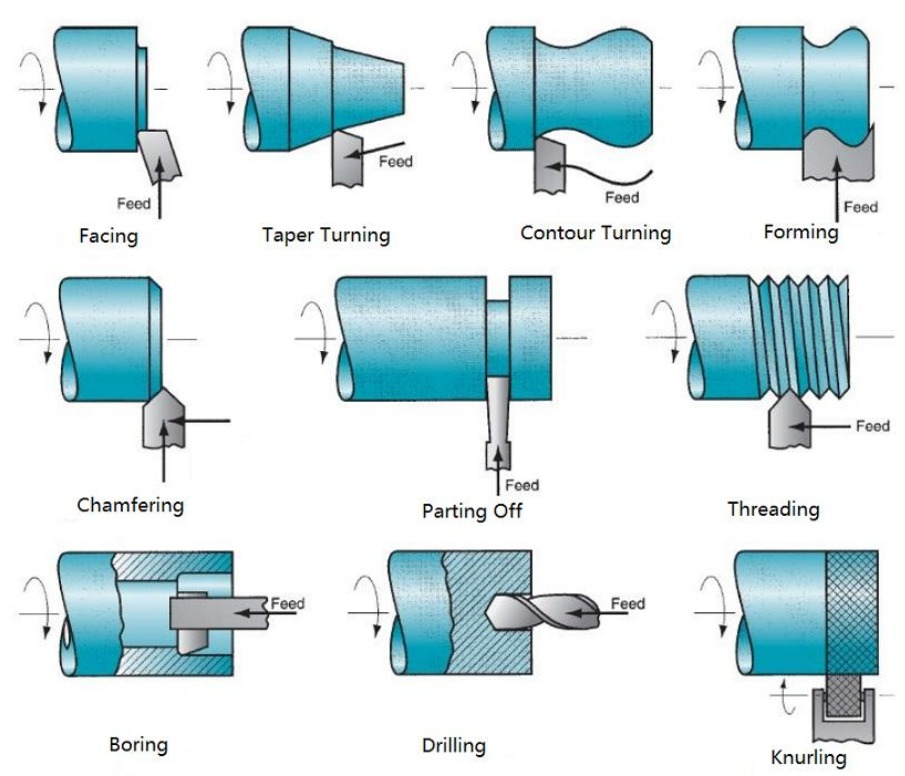
\includegraphics[width=0.5\textwidth]{img/operations.jpeg} 
  \caption{Operations of Engine Lathe} 
  \label{fig:operations}
\end{figure}

\begin{figure}[htbp]
  \centering
  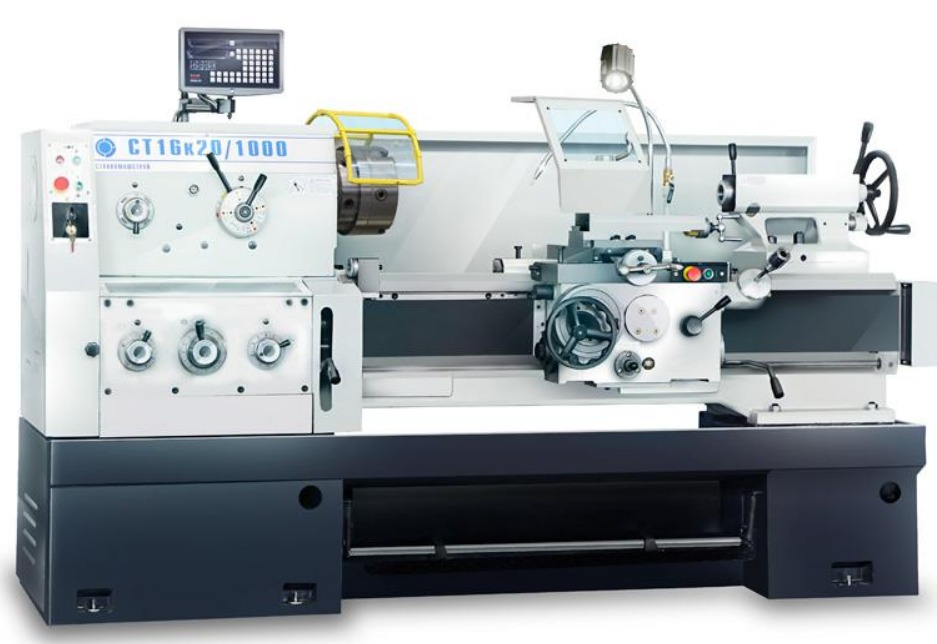
\includegraphics[width=\textwidth]{img/engine_lathe.jpeg} 
  \caption{Engine Lathe Machine} 
  \label{fig:engine_lathe}
\end{figure}

\begin{figure}[htbp]
  \centering
  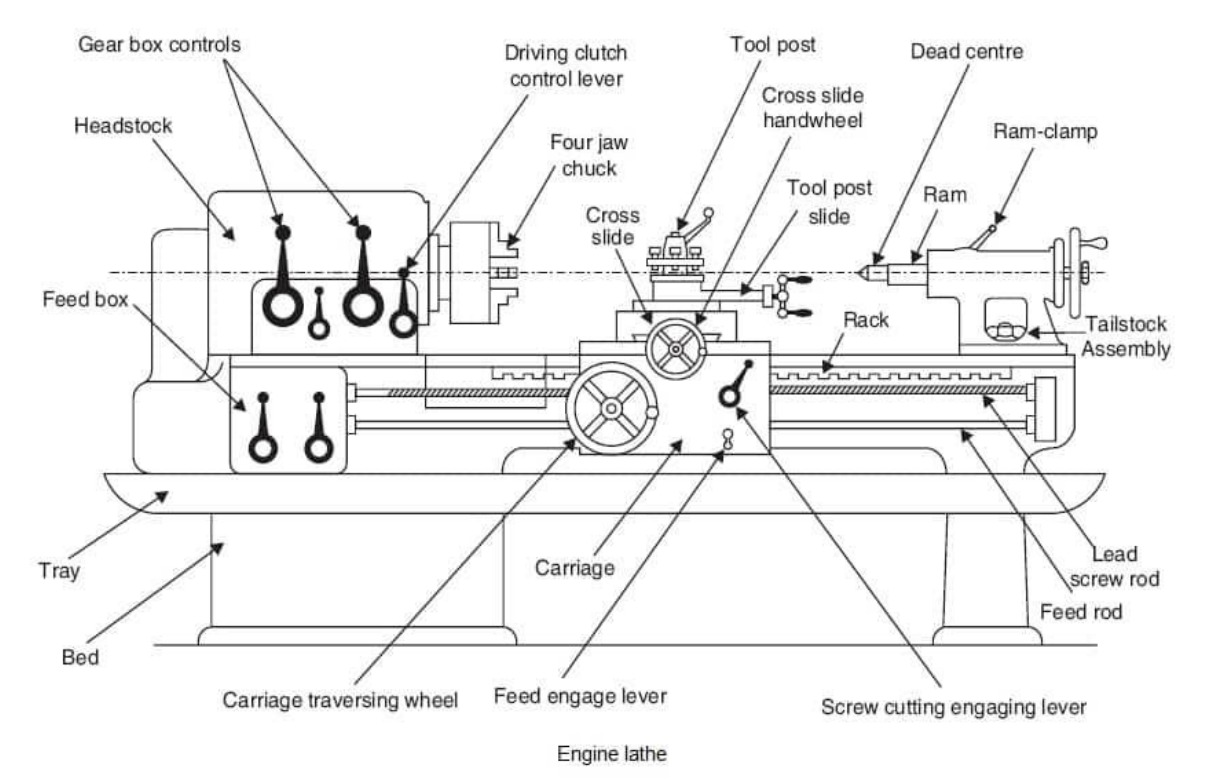
\includegraphics[width=\textwidth]{img/diagram.jpeg} 
  \caption{A Schematic Diagram Engine Lathe} 
  \label{fig:engine_lathe_diagram}
\end{figure}


\subsubsection*{Bed}
\begin{itemize}
  \item Main body of the machine
  \item All the main components are bolted on it 
  including the headstock, tailstock, carriage 
  etc.
  \item Usually made of cast iron due to its high 
  compressive strength
  \item Contains guide ways that guides the 
  carriage and tailstock
\end{itemize}

\subsubsection*{Headstock}
\begin{itemize}
  \item Provides the rotational power for the lathe’s operations
  \item Holds the speed gear box, spindle, chuck, gear speed control levers, and feed controllers
  \item Made up of cast iron
  \item Usually positioned on the left side of the bed
\end{itemize}

\subsubsection*{Spindle}
\begin{itemize}
  \item A hollow shaft on which the chuck is mounted and rotated
  \item Made from good quality alloy steel and is heat treated
  \item Threads, tapers, etc. are made at one end of the spindle to which holding devices can be attached
\end{itemize}

\subsubsection*{Chuck}
\begin{itemize}
  \item Used to hold workpiece
  \item Usually of 2 types – 3 Jaw Self centering Chuck and 4 Jaw Independent Chuck
  \item Collet chuck is used for some special purpose cases
\end{itemize}

\subsubsection*{Tailstock}
\begin{itemize}
  \item Support the loose end of the workpiece or a job 
  while machining
  \item Hold the cutting tools such as drill chucks, drills, 
  reamers etc.
  \item Can slide on the bed guideways and can be clamped 
  in any position
  \item Center can be live or dead; live center rotates with 
  workpiece while dead center does not
\end{itemize}

\subsubsection*{Carriage}
\begin{itemize}
  \item Located between headstock and tailstock 
  \item Move the tool post along the bed
  \item Impart the feed movement along z axis of 
  lathe machine from lead screw and feed rod
  \item Consists of 7 main parts – (i) Apron (ii) Saddle 
  (iii) Cross slide (iv) Swivel plate (v) Compound 
  Rest (vi) Top slide (vii) Tool post
\end{itemize}


\begin{figure}
  \centering

  \subfigure[Bed]{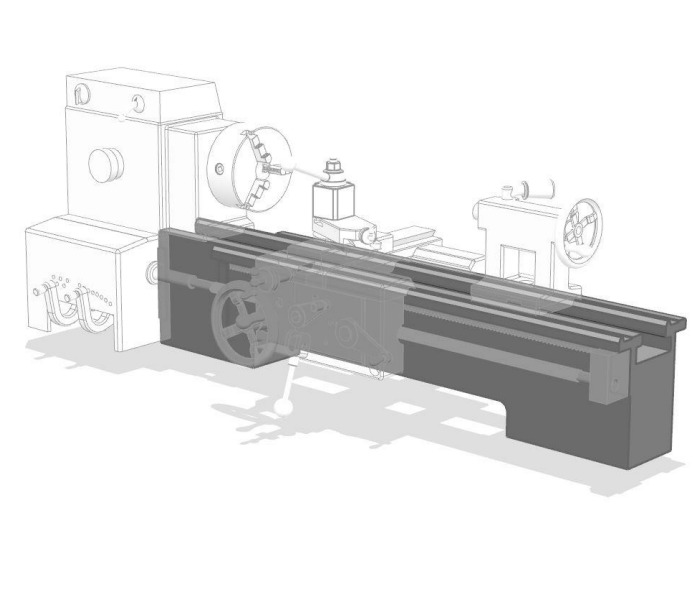
\includegraphics[width=0.3\linewidth]{img/bed.jpeg}}
  \hfill
  \subfigure[Headstock]{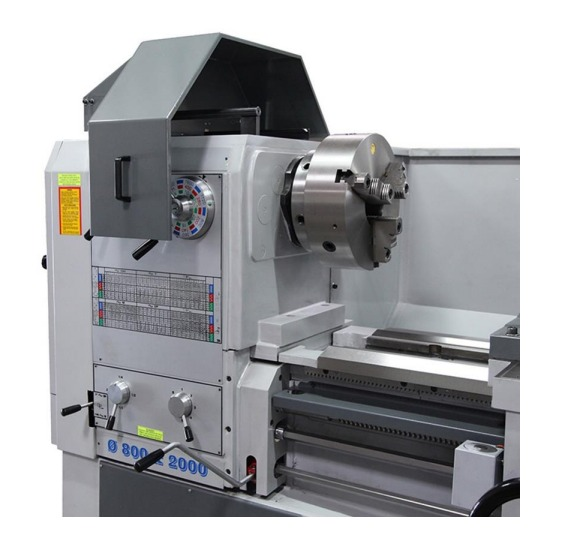
\includegraphics[width=0.3\linewidth]{img/headstock.jpeg}}
  \hfill
  \subfigure[Spindle]{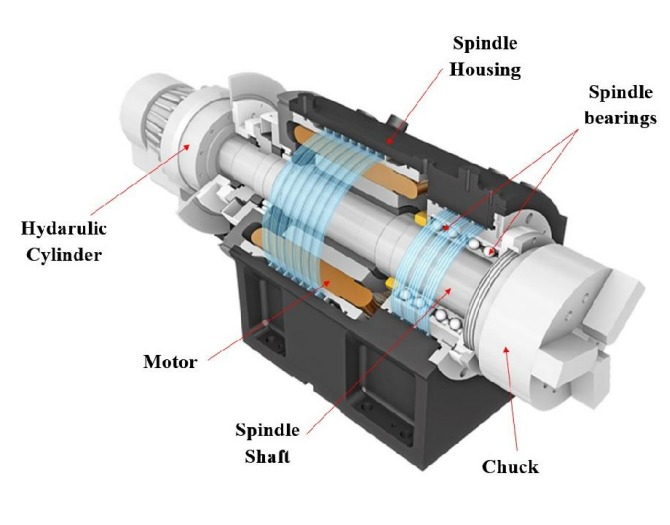
\includegraphics[width=0.3\linewidth]{img/spindle.jpeg}}

  \vspace{0.5cm}

  \subfigure[Chuck]{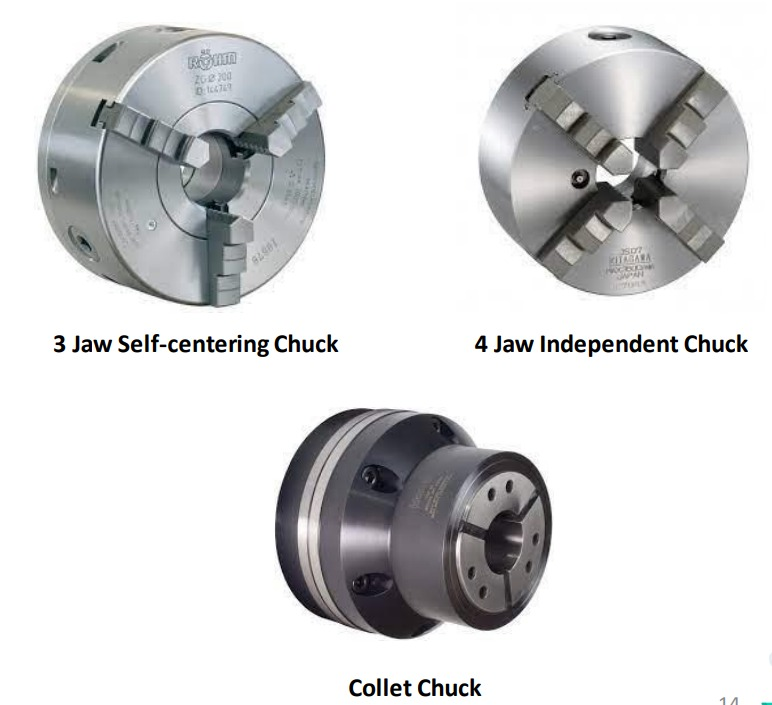
\includegraphics[width=0.3\linewidth]{img/chuck.jpeg}}
  \hfill
  \subfigure[Tailstock]{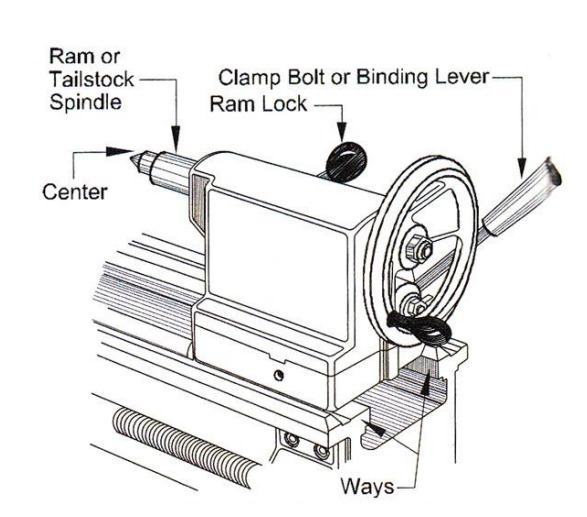
\includegraphics[width=0.3\linewidth]{img/tailstock.jpeg}}
  \hfill
  \subfigure[Carriage]{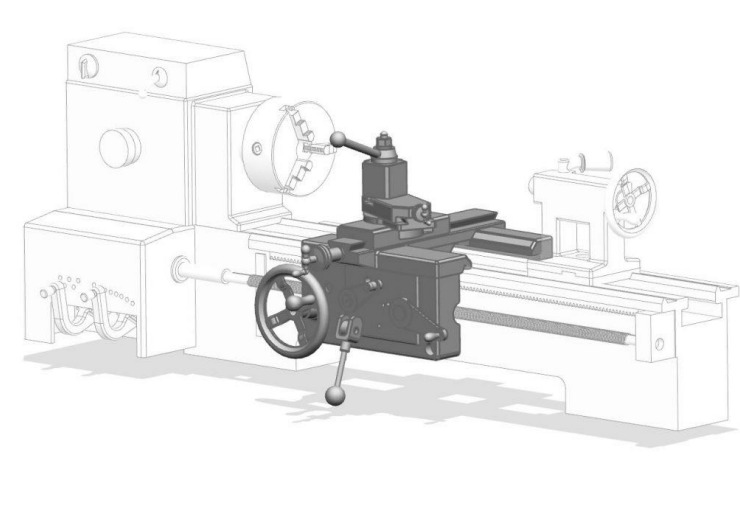
\includegraphics[width=0.3\linewidth]{img/carriage.jpeg}}

  \caption{Components of Engine Lathe}
\end{figure}

\subsubsection*{Apron}
\begin{itemize}
  \item Located on the front face of the carriage 
  \item Responsible for receiving power from the lead screw or the feed rod
  \item Transfer the power to move either the carriage itself or the cross slide
\end{itemize}

\subsubsection*{Saddle}
\begin{itemize}
  \item A ‘H’ shaped part of the carriage that rides on 
  the bed
  \item Responsible for supporting cross slide 
  movements
\end{itemize}

\subsubsection*{Cross Slide}
\begin{itemize}
  \item Mounted on top surface of saddle
  \item Allow the movement of a tool post at a right angle to the bed guideways during machining (along x axis of lathe machine)
\end{itemize}

\subsubsection*{Swivel Plate}
\begin{itemize}
  \item Mounted on cross slide
  \item Allow the compound rest thus the tool post to rotate as per requirement
  \item Graduations of degrees are marked on the swivel plate to facilitate rotation
\end{itemize}

\subsubsection*{Compound Rest}
\begin{itemize}
  \item Mounted on swivel plate
  \item It is a stationary part on which the top slide moves
  \item Direction of the compound rest is set by the direction of swivel plate
\end{itemize}

\subsubsection*{Top Slide}
\begin{itemize}
  \item Mounted on compound rest
  \item Movement of this part provides the depth of 
  cut of the corresponding lathe operation
  \item Tool post is mounted on top of it
\end{itemize}

\subsubsection*{Tool Post}
\begin{itemize}
  \item Mounted on top slide
  \item Used to hold the tools at the correct position with rigidity
  \item Main tool holder is known as square turret which is used for typical lathe cutting tool
  \item Back tool holder is used for grooving operations
\end{itemize}

\subsubsection*{Speed Gear Box}
\begin{itemize}
  \item Gear train positioned inside headstock
  \item Responsible for precise rotational speed of spindle
  \item Has a number of available standard rotational speeds 
  \item Takes the power from main motor via belt pulley mechanism
\end{itemize}

\subsubsection*{Feed Gear Box}
\begin{itemize}
  \item Gear train positioned below the speed gear box
  \item Responsible for feed movements of carriage and cross slide
  \item Receives the power from spindle via change gear box
  \item Provides motion to lead screw and feed rod
\end{itemize}

\subsubsection*{Lead Screw \& Feed Rod}
\begin{itemize}
  \item  Responsible for transferring feed motion from feed gear box to carriage
  \item Engage with carriage via apron 
  \item Lead screw is used for high feed rate operations like threading while feed rod is used for low feed rate operations like turning
\end{itemize}

\begin{figure}
  \centering

  \subfigure[Apron]{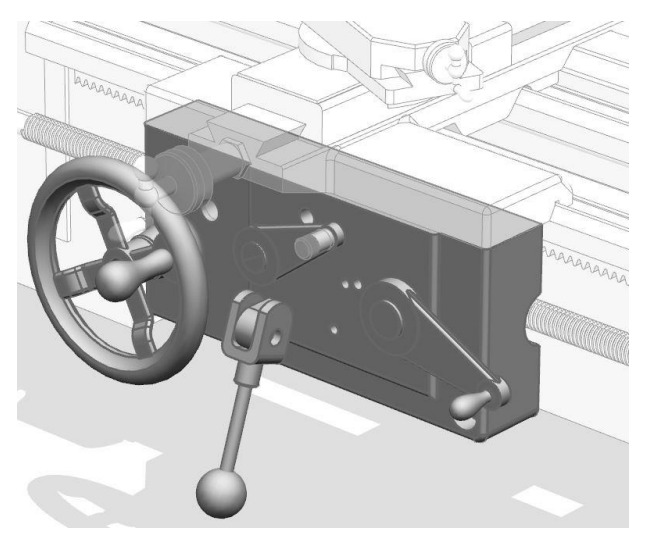
\includegraphics[width=0.24\linewidth]{img/apron.jpeg}}
  \hfill
  \subfigure[Saddle]{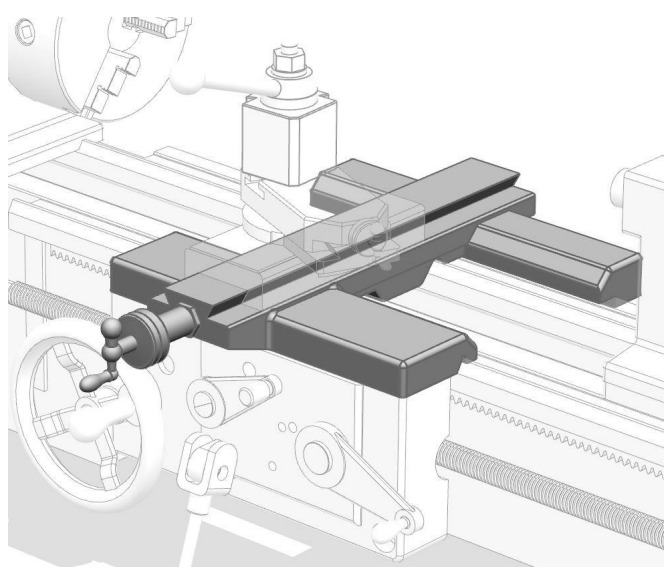
\includegraphics[width=0.24\linewidth]{img/saddle.jpeg}}
  \hfill
  \subfigure[Cross Slide]{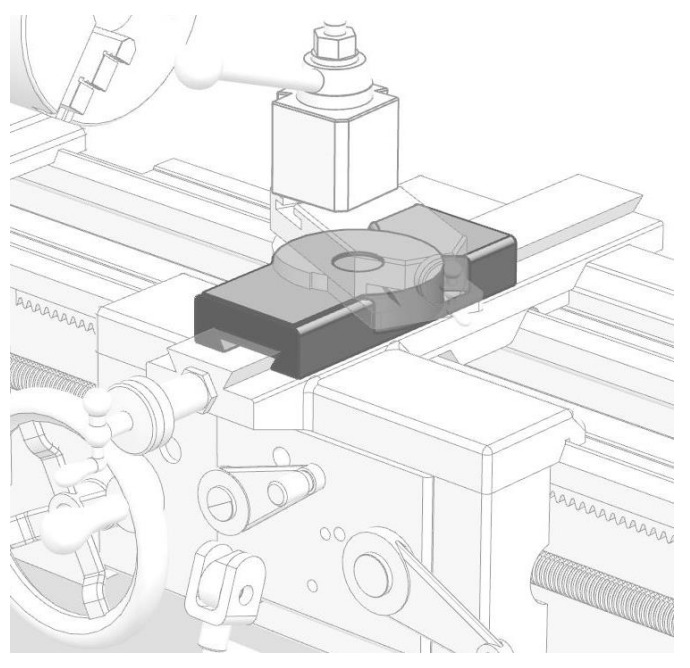
\includegraphics[width=0.24\linewidth]{img/cross_slide.jpeg}}
  \subfigure[Swivel Plate]{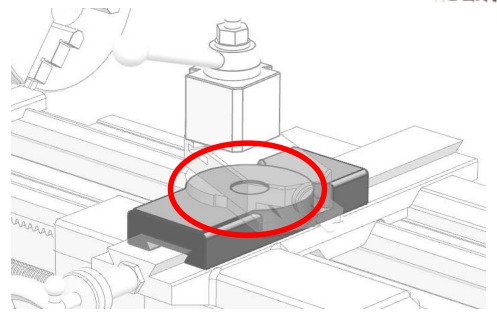
\includegraphics[width=0.24\linewidth]{img/swivel_plate.jpeg}}

  \vspace{0.2cm}

  \subfigure[Speed Gear Box]{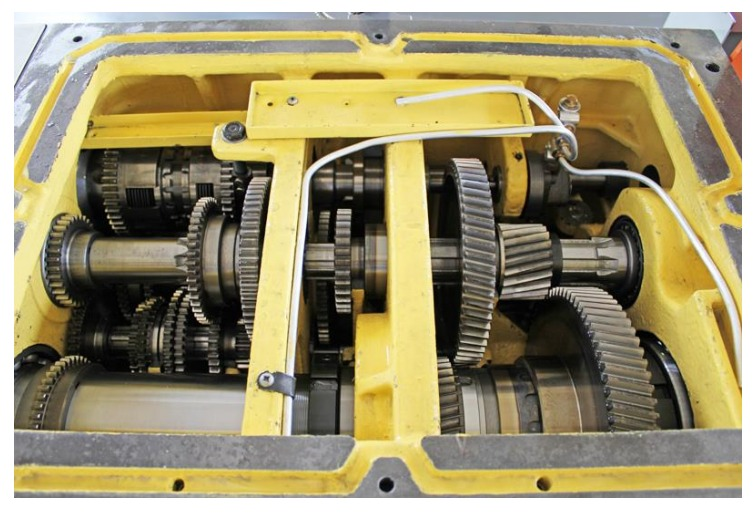
\includegraphics[width=0.24\linewidth]{img/speed_gear_box.jpeg}}
  \hfill
  \subfigure[Feed Gear Box]{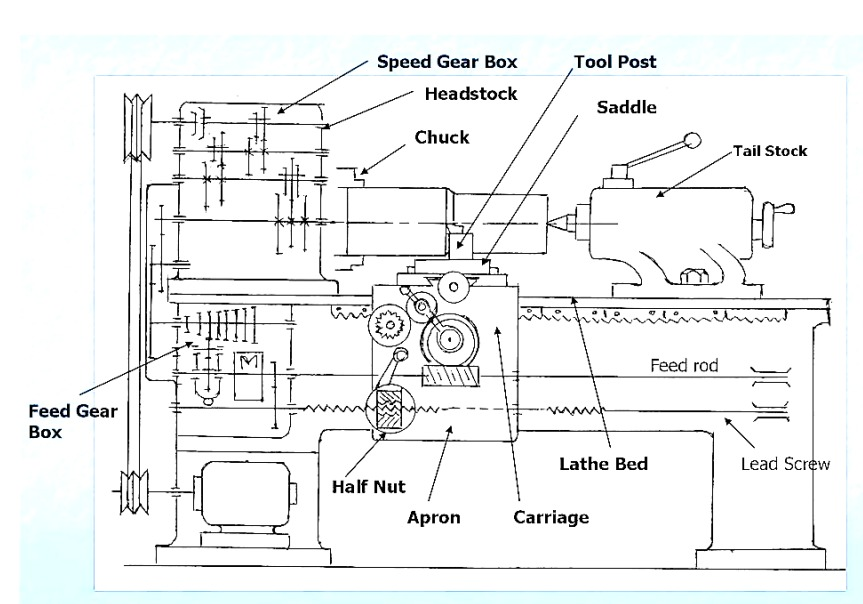
\includegraphics[width=0.24\linewidth]{img/feed_gear_box.jpeg}}
  \hfill
  \subfigure[Tool Post]{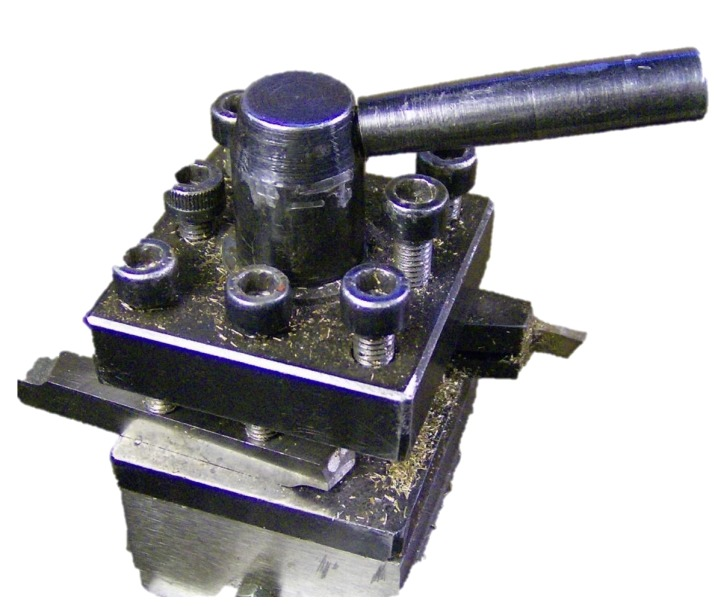
\includegraphics[width=0.24\linewidth]{img/tool_post.jpeg}}
  \subfigure[Lead Screw]{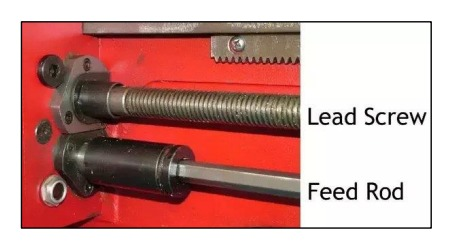
\includegraphics[width=0.24\linewidth]{img/lead_screw.jpeg}}
  \caption{Components of Engine Lathe}
\end{figure}

\vspace*{0.5cm}
\begin{figure}[ht]
  \subsubsection*{Axis of Rotation}
  \centering
  \begin{minipage}{0.45\linewidth}
      \begin{itemize}
        \item Along the spindle → z axis 
        \item up to down → y axis 
        \item front to back → x axis 
      \end{itemize}
  \end{minipage}%
  \begin{minipage}{0.55\linewidth}
      \centering
      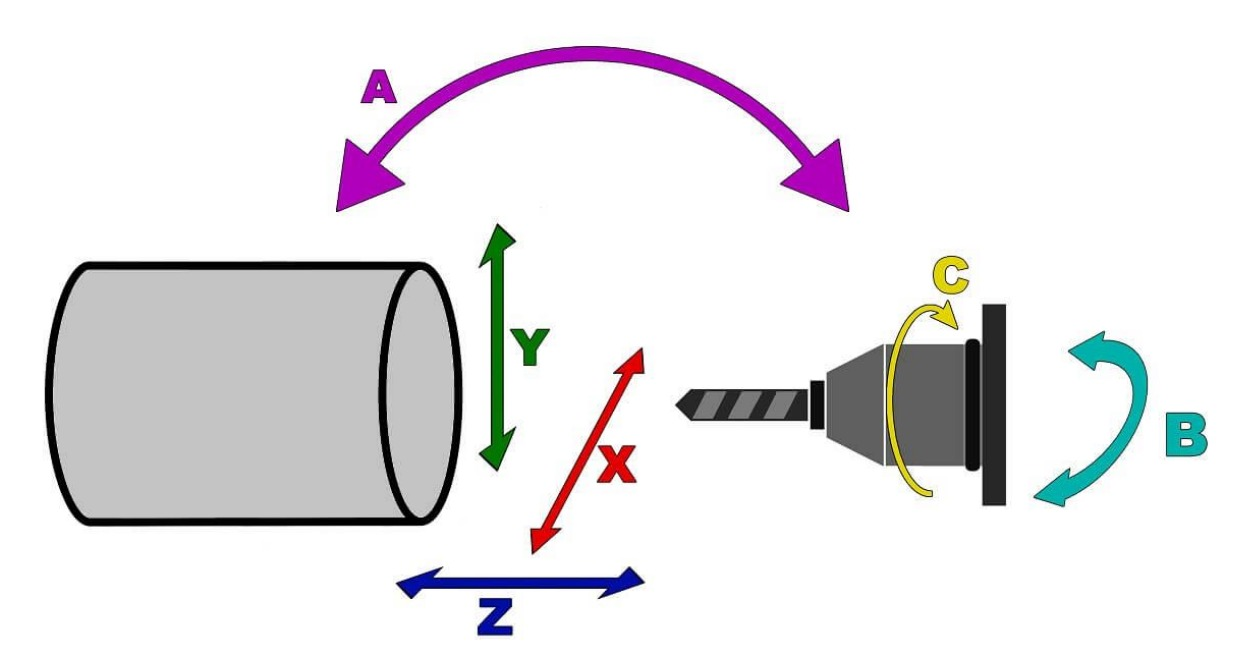
\includegraphics[width=\linewidth]{img/axis.jpeg}
      \caption{Axis of Rotation in engine lathe}
      \label{fig:axis}
  \end{minipage}
\end{figure}




\newpage

\section{Lecture 2: Apron Mechanism \& Short Gear Train}
\hfill Date: 12/06/2023

\subsection*{Apron Mechanism}
\begin{itemize}
  \item  Apron mechanism is the mechanism of power 
  transmission from feed rod to apron
  \item Carriage moves using rack and pinion 
  mechanism
  \item Feed rod is engaged with the worm gear 
  using key slot mechanism
  \item Automatic motion can be provided to 
  longitudinal and cross direction using power 
  clutch system
\end{itemize}

\subsection*{Half Nut Mechanism}
\begin{itemize}
  \item Lead screw is engaged with apron using half nut mechanism unlike key slot mechanism of feed rod
  \item The half nut is mounted on the back side of the apron
  \item Half nut can be engaged/disengaged using a lever
\end{itemize}


\begin{figure}[ht]
  \subsection*{Main Dimension of Engine Lathe}
  \centering
  \begin{minipage}{0.5\linewidth}
    \begin{enumerate}
      \item Height of centers over bed
      \item Maximum diameter of workpiece accommodated over the bed (most important)
      \item Maximum diameter of workpiece accommodated over the carriage
      \item Maximum diameter of workpiece accommodated over the gap
      \item Maximum distance between centers
      \item Length of the bed
      \item No. of speeds and feeds
    \end{enumerate}
  \end{minipage}%
  \begin{minipage}{0.5\linewidth}
    \centering
    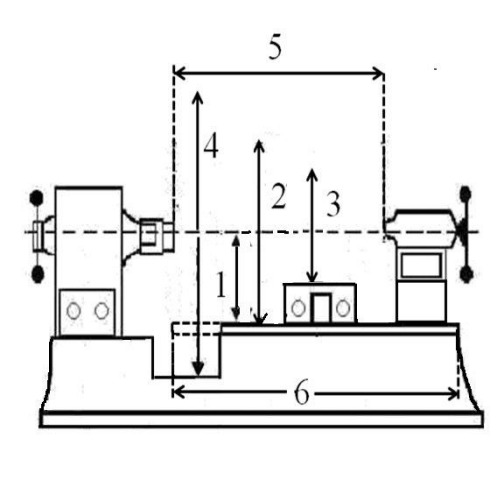
\includegraphics[width=\linewidth]{img/dimension.jpeg}
    \caption{Main Dimension of engine lathe}
  \end{minipage}
\end{figure}

\subsection*{Short Gear Train}
\begin{figure*}[h]
  \centering
  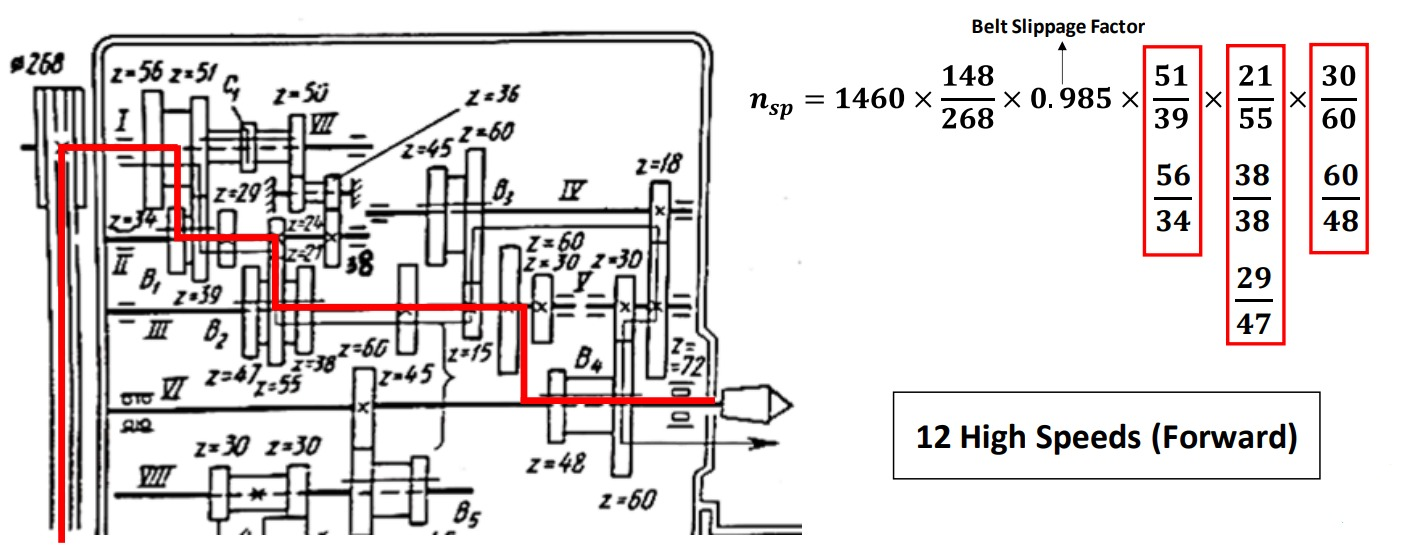
\includegraphics[width=\linewidth]{img/short_gear_disengaged.jpeg}
  \caption{Forward Rotation (without back gear) $\rightarrow$ $C_1$ Disengaged}
\end{figure*}

\begin{figure*}[h] 
  \centering
  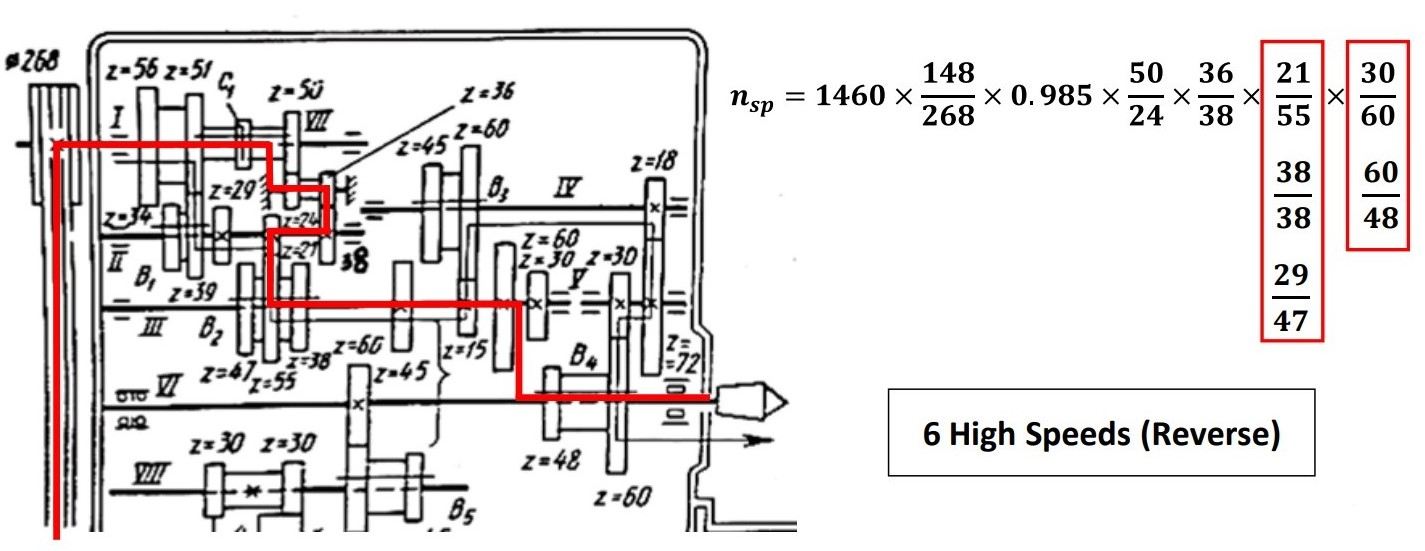
\includegraphics[width=\linewidth]{img/short_gear_engaged.jpeg}
  \caption{Forward Rotation (with back gear) $\rightarrow$ $C_1$ Engaged}
\end{figure*}

\end{document}
